\documentclass[dvipsnames]{beamer}
\usepackage{polyglossia}
\usepackage{multicol}
\setdefaultlanguage{slovak}
\setbeamertemplate{caption}{\raggedright\insertcaption\par}
\setbeamerfont{caption}{size=\footnotesize}
\setbeamerfont{section in toc}{size=\small}
\setbeamerfont{subsection in toc}{size=\footnotesize}
\setbeamerfont{subsubsection in toc}{size=\scriptsize}
\setlength{\belowcaptionskip}{-13pt}
\setlength{\abovecaptionskip}{-5pt}
\setlength\intextsep{-10cm}
\definecolor{bgc}{RGB}{250,250,250}
\definecolor{tc}{RGB}{0,0,100}
\definecolor{su}{RGB}{0,100,0}
\definecolor{g}{RGB}{0,210,10}
\urlstyle{same}
\setlength{\columnseprule}{0.1pt}
\setbeamercolor{sectionColor}{fg=white,bg=RoyalBlue}
\setbeamercolor{background canvas}{bg=bgc,fg=white}
\setbeamercolor{normal text}{fg=tc}
\setbeamercolor{frametitle}{fg=ForestGreen}
\hypersetup{
    colorlinks=true,
    urlcolor={cyan},
    linkcolor=,
    pdfpagemode=FullScreen,
    }
\setbeamertemplate{section page}
{
    \begingroup
    \begin{beamercolorbox}[sep=12pt,center]{sectionColor}%
        \usebeamerfont{section title}\insertsection\par
    \end{beamercolorbox}
    \endgroup
}
\addtobeamertemplate{frametitle}{}{\vspace{-1.5em}}
\addtobeamertemplate{itemize subbody begin}{\scriptsize}

\title{Umenie a kultúra v 17. a 18. storočí}
\author{Adam Jenča a  Alica Jenčová, Sekunda}
\begin{document}
\begin{frame}
	\titlepage
\end{frame}
\begin{frame}
	\frametitle {Obsah}
	\begin{multicols}{2}
		\tableofcontents
	\end{multicols}
\end{frame}
\section{Hudba}
\frame{\sectionpage}
\begin{frame}{Barok}
	\subsection{Barok}
	\begin{itemize}
		\item Začiatok hudobného novoveku
		\item Odčlenenie inštrumentálnej hudby
		\item Dôraz na polyfóniu
	\end{itemize}
	\begin{columns}
		\column{0.5\textwidth}
		
		\kern0pt
		\begin{figure}
		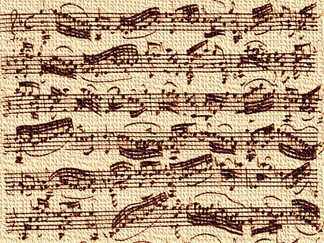
\includegraphics[scale=1.5]{baroko}
		\caption{Notový zápis z baroka}
		\end{figure}%
		
		\column{0.5\textwidth}
		\begin{figure}
			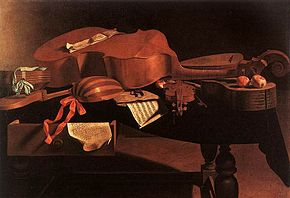
\includegraphics[scale=1.5]{in}
			\caption{Odčlenenie inštrumentálnej hudby}
		\end{figure}
	\end{columns}

\end{frame}
\begin{frame}{\small \textcolor{g}{Barok} / \Large Nástroje}
	\subsubsection{Nástroje}
	\begin{itemize}
		\item Najvyužívanejšie:	
		\begin{itemize}
		\item Flauta
		\item Trúbka
		\item Organ
		\item Čembalo
		\item Sláčikový orchester
		\end{itemize}
	\end{itemize}
	\begin{columns}
	\kern0pt
		\column{0.5\textwidth}
	\begin{figure}
		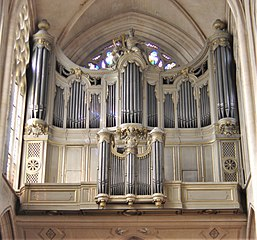
\includegraphics[scale=0.25]{organ}
		\caption{Organ}
	\end{figure}%
	\begin{figure}
		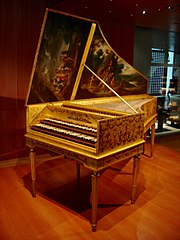
\includegraphics[scale=0.25]{cembalo}
		\caption{Čembalo}
	\end{figure}%
	\column{0.5\textwidth}
	
		\begin{figure}
			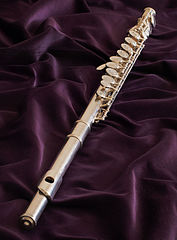
\includegraphics[scale=1.5]{flauta}
		\caption{Flauta}
	\end{figure}%
		\begin{figure}
			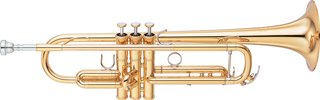
\includegraphics[scale=0.3]{truba}
		\caption{Trúbka}
	\end{figure}%

	\end{columns}
\end{frame}
\begin{frame}{\small \textcolor{g}{Barok} / \Large Skladatelia}
	\subsubsection{Skladatelia}
	\begin{columns}
	\column{0.5\textwidth}
	
	\begin{itemize}
		\item Raný barok
		\begin{itemize}
			\item C. Monteverdi
		\end{itemize}
		\item Vrcholný  barok
		\begin{itemize}
			\item J. S. Bach - \href{https://www.gtsforum.xyz/organ.mp3}{ukážka}
			\item G. F. Händel
			\item A. Vivaldi - \href{https://www.gtsforum.xyz/vivaldi.mp3}{ukážka}
		\end{itemize}

	\end{itemize}
	\column{0.5\textwidth}
	\begin{figure}
		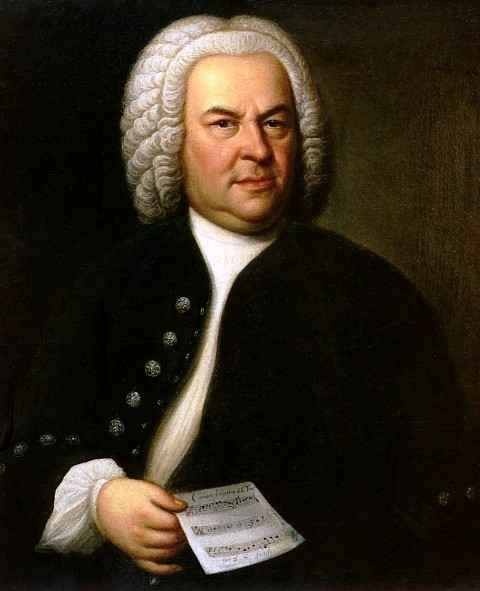
\includegraphics[scale=0.75]{bach}
		\caption{Johann Sebastian Bach}
	
	\end{figure}%
	\begin{figure}
		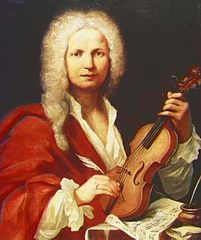
\includegraphics[scale=1.75]{vivaldi}
		\caption{Antonio Vivaldi}
	\end{figure}

	\end{columns}
\end{frame}
\begin{frame}{Klasicizmus}
	\subsection{Klasicizmus}
	\begin{itemize}
		\item Vznik a rozvoj sonátovej formy
		\item Rozlišovanie dur/mol
		\item Vznik symfónie
		
	\end{itemize}
	\begin{figure}
		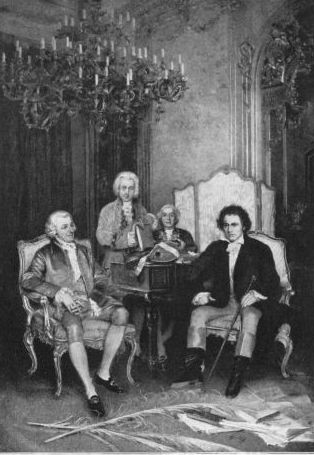
\includegraphics[scale=0.3]{klasmu}
		\caption{Najväčší skladatelia klasicizmu: Haydn, Mozart a Beethoven}
	\end{figure}
\end{frame}
\begin{frame}{\small \textcolor{g}{Klasicizmus} / \Large Skladatelia}
	\subsubsection{Skladatelia}
	\begin{columns}
	\column{0.7\textwidth}

	\begin{itemize}
		\item Joseph Haydn - \href{https://www.gtsforum.xyz/haydn.mp3}{ukážka}
		\item Wolfgang Amadeus Mozart - \href{https://www.gtsforum.xyz/mozart.mp3}{ukážka}
		\item Ludwig van Beethoven - \href{https://www.gtsforum.xyz/beethoven.mp3}{ukážka}
		\item Niccolò Paganini - \href{https://www.gtsforum.xyz/paganini.ogg}{ukážka}
		\item Christoph  Willibald Gluck - \href{https://www.gtsforum.xyz/gluck.ogg}{ukážka}
	\end{itemize}
	\column{0.3\textwidth}
		\begin{figure}
			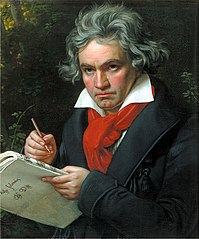
\includegraphics[scale=0.45]{beethoven}
			\caption{L. van Beethoven}
		\end{figure}
		\begin{figure}
			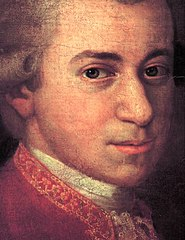
\includegraphics[scale=0.45]{mozart}
			\caption{W. A. Mozart}
		\end{figure}

	\end{columns}
\end{frame}
\section{Literatúra}
\frame{\sectionpage}

\begin{frame}{17. storočie}
	\subsection{17. storočie}	
	\begin{itemize}
		\item Renesancia -> prostredie pre nové myšlienky
		\item ,,Čo viem ?'' = skepticizmus
		\item Prechod do modernej doby + nárast významu vedy = kríza v umení
		\begin{minipage}[t]{0.4\textwidth}
		\kern0pt
		
		\begin{figure}
			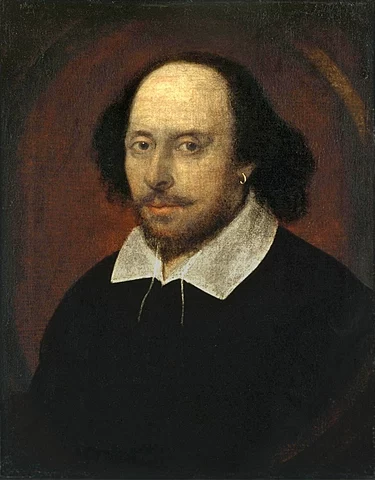
\includegraphics[scale=0.2]{pivo}
			\caption{William Shakespeare}
		\end{figure}
		\end{minipage}%
		\begin{minipage}[t]{0.6\textwidth}
		\kern0pt

		\begin{figure}
			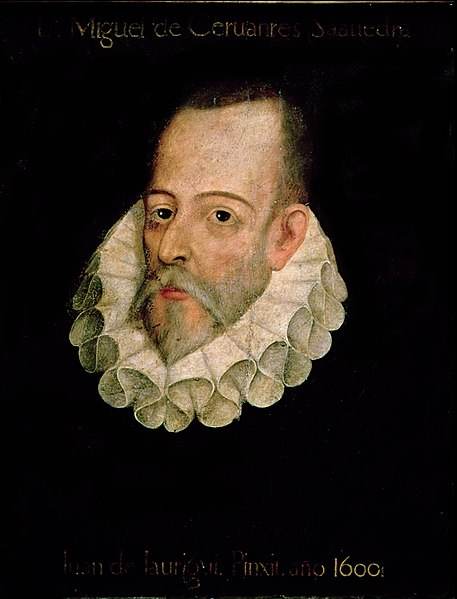
\includegraphics[scale=0.1605]{cervo}
			\caption{Miguel de Cervantes}
		\end{figure}
		\end{minipage}
	\end{itemize}
\end{frame}
\begin{frame}{\small \textcolor{g}{17. storočie} / \Large Významní spisovatelia 17. storočia}
	\subsubsection{Významní spisovatelia 17. storočia}
	\begin{columns}
	\column{0.6\textwidth}

	\begin{itemize}
		\item John Milton
		\bigskip
		\item Lope de Vega
		\bigskip
		\item René Descartes
		\bigskip
		\item Molière
	\end{itemize}
	\column{0.4\textwidth}
	\begin{figure}
		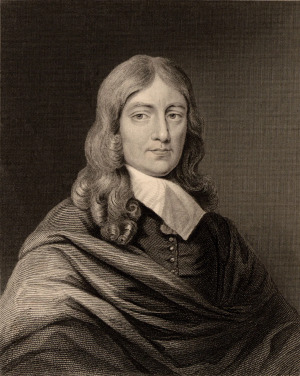
\includegraphics[scale=0.25]{milton}
		\caption{John Milton}
	\end{figure}%
	\begin{figure}
		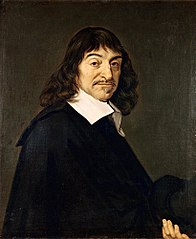
\includegraphics[scale=0.35]{dekart}
		\caption{René Descartes}
	\end{figure}

	\end{columns}
\end{frame}
\begin{frame}

\frametitle{18. storočie}
\subsection{18. storočie}
\begin{itemize}
	\item Literatúra ovplyvnená osvietenstvom
	\item Vznik moderného románu
	\item Encyklopédia
\end{itemize}
\begin{minipage}[t]{0.5\textwidth}
	\kern0pt
	\begin{figure}
		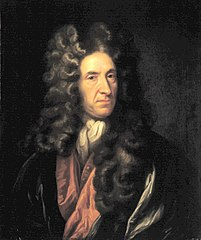
\includegraphics[scale=0.4]{defoe}
		\caption{Daniel Defoe}
	\end{figure}
\end{minipage}%
\begin{minipage}[t]{0.5\textwidth}
	\kern0pt
	\begin{figure}
		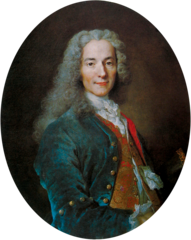
\includegraphics[scale=0.4]{voltik}
		\caption{Voltaire}
	\end{figure}
\end{minipage}


\end{frame}

\begin{frame}{\small{\textcolor{g}{18. storočie}} / \Large Významní spisovatelia 18. storočia}
	
\subsubsection{Významní spisovatelia 18. storočia}
\begin{columns}
	
\column{0.6\textwidth}
\begin{itemize}
	\item Jonathan Swift
	\bigskip
	\item J.W. von Goethe
	\bigskip
	\item Denis Diderot
	\bigskip
	\item J.J. Rosseau
\end{itemize}
\column{0.4\textwidth}
	\begin{figure}
		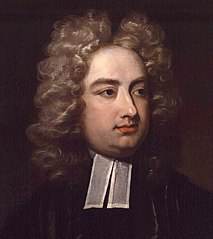
\includegraphics[scale=0.4]{swift}
		\caption{Jonathan Swift}
	\end{figure}%
	\begin{figure}
		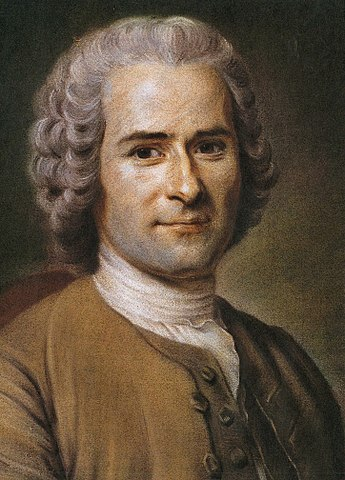
\includegraphics[scale=0.225]{rosseau}
		\caption{J.J. Rosseau}
	\end{figure}

	\end{columns}
\end{frame}


\section{Architektúra}
\frame{\sectionpage}
\begin{frame}{Baroková architektúra}
	\subsection{Baroková architektúra}
	\begin{itemize}
		\item Barok - ,,vzbura'' proti prísnym pravidlám renesancie
		\item Vznik: 17. storočie , Taliansko - začatá katolíkmi
		\item Dekoratívne prvky
		\item Prehnaný dôraz na zložitosť
	\end{itemize}
		\begin{figure}
			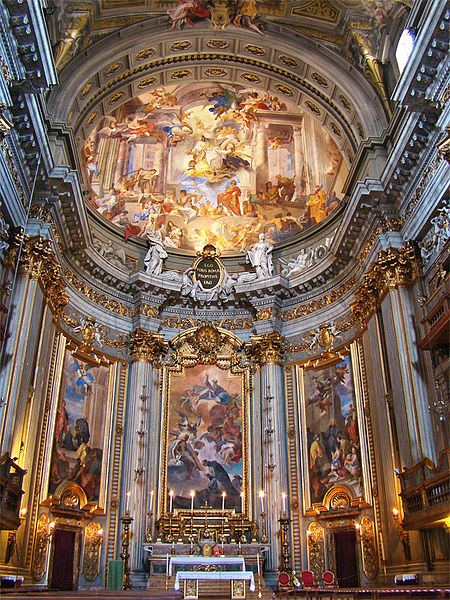
\includegraphics[scale=0.3]{loyola}
			\caption{Interiér kostola sv. Ignáca z Loyoly, Rím}
		\end{figure}
\end{frame}
\begin{frame}{\small \textcolor{g}{Baroková architektúra} / \Large Raný barok}
	\subsubsection{Raný barok}
	\begin{itemize}
		\item Odpoveď na reformáciu
		\item Objednávatelia - Jezuiti
		\item Stavby
		\begin{itemize}
			\item \textcolor{BurntOrange}{Carlo Maderno} - Fasáda Baziliky Sv. Petra
				\item \textcolor{BurntOrange}{Giacomo della Porta} - Kostol Il Gesú
				\item \textcolor{BurntOrange}{Salomon de Brosse} - Luxemburský palác
				\item \textcolor{BurntOrange}{Louis le Vau} - château Vaux-le-Vicomte
				\item \textcolor{BurntOrange}{Giovanni Maria Bernardoni} - Kostol Sv. Petra a Pavla
		\end{itemize}
		\begin{columns}
			\column{0.5\textwidth}
			\kern0pt
			\begin{figure}
				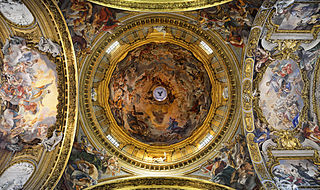
\includegraphics[scale=0.5]{gesu}
				\caption{Strop kostola Il Gesú}
			\end{figure}%
			\column{0.5\textwidth}
			\begin{figure}
				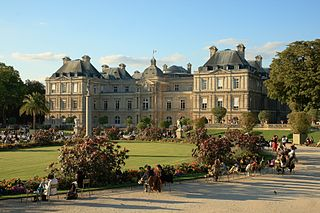
\includegraphics[scale=3.5]{lux}
				\caption{Luxemburský palác}
			\end{figure}
		\end{columns}
	\end{itemize}
\end{frame}
\begin{frame}{\small \textcolor{g}{Baroková architektúra} / \Large Vrcholný barok}
	\subsubsection{Vrcholný barok}
	\begin{itemize}
		\item Patrón: Pápež \textcolor{BurntOrange}{Urban VIII.}
		\item Hlavný cirkevný architekt: \textcolor{BurntOrange}{Gian Lorenzo Bernini}
		\item Stavby:
		\begin{itemize}
			\item \textcolor{BurntOrange}{Bernini} - Barokové centrum Ríma
			\item \textcolor{BurntOrange}{Francesco Borromini} - Kostol San Carlo alle Quattro Fontane
			\item \textcolor{BurntOrange}{Maderno}, \textcolor{BurntOrange}{Bernini} a \textcolor{BurntOrange}{Borromini} - Palác Barberiniovcov
			\item \textcolor{BurntOrange}{Baldassare Longhena} - Kostol Santa Maria della Salute
			\item \textcolor{BurntOrange}{Pietro da Cortona} - Kostol Santi Luca e Martina
		\end{itemize}
		\begin{columns}
			\column{0.33\textwidth}
			\kern0pt
			\begin{figure}
				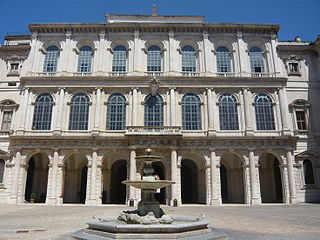
\includegraphics[scale=0.325]{barberini}
				\caption{Palác Barberiniovcov}
			\end{figure}%
			\column{0.33\textwidth}
			\begin{figure}
				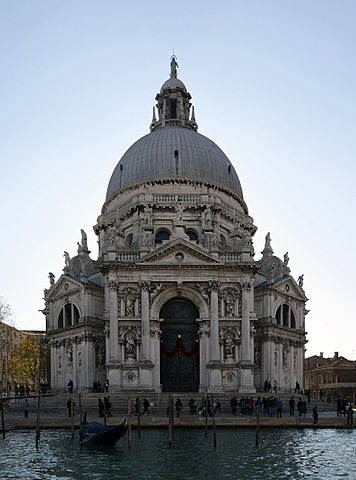
\includegraphics[scale=0.225]{salute}
				\caption{Santa Maria della Salute}
			\end{figure}%
			\column{0.33\textwidth}
			\begin{figure}
				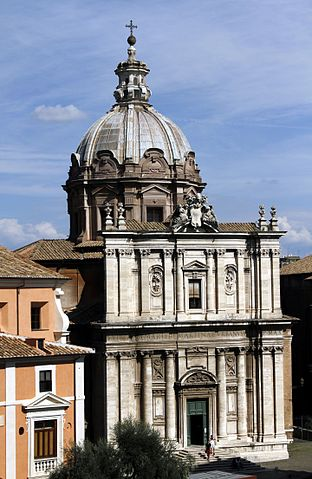
\includegraphics[scale=0.225]{slem}
				\caption{ Santi Luca e Martina}
			\end{figure}


		\end{columns}
	\end{itemize}
\end{frame}
\begin{frame}{\small \textcolor{g}{Baroková architektúra} / \Large Neskorý barok}
	\subsubsection{Neskorý barok}
	\begin{itemize}
		\item Vznik rokoka - orientálne vplyvy
		\item Španielsko - Churriguerizmus -> ,,ultrabarok''
		\item Stavby:
		\begin{itemize}
			\item \textcolor{BurntOrange}{Filippo Juvarra} - Bazilika na Superge
			\item \textcolor{BurntOrange}{J. Hardouin-Mansart} - Zrkadlová sieň a kaplnka vo Versailles
			\item \textcolor{BurntOrange}{Fischer von Erlach} - Kalskirche
			\item \textcolor{BurntOrange}{Jose Benito de Churriguera} - Oltár v Segovijskej Katedrále
		\end{itemize}
	\end{itemize}
	\vskip -4mm
	\begin{columns}
		\kern0pt
		\column{0.33\textwidth}
		\begin{figure}
			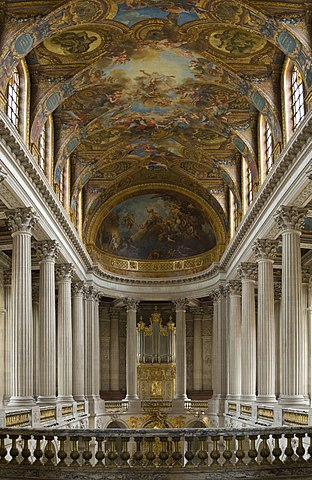
\includegraphics[scale=0.25]{verzajl}
			\vskip 0.5mm
			\caption{\centering Kaplnka Versaillského Paláca}
		\end{figure}%
		\column{0.33\textwidth}
		\begin{figure}
			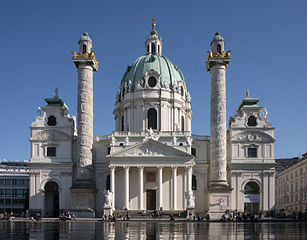
\includegraphics[scale=1.5]{karlskirchw}
			%\vskip 0.5mm
			\caption{\centering Karlskirche}
		\end{figure}%
		\column{0.33\textwidth}
		\begin{figure}
			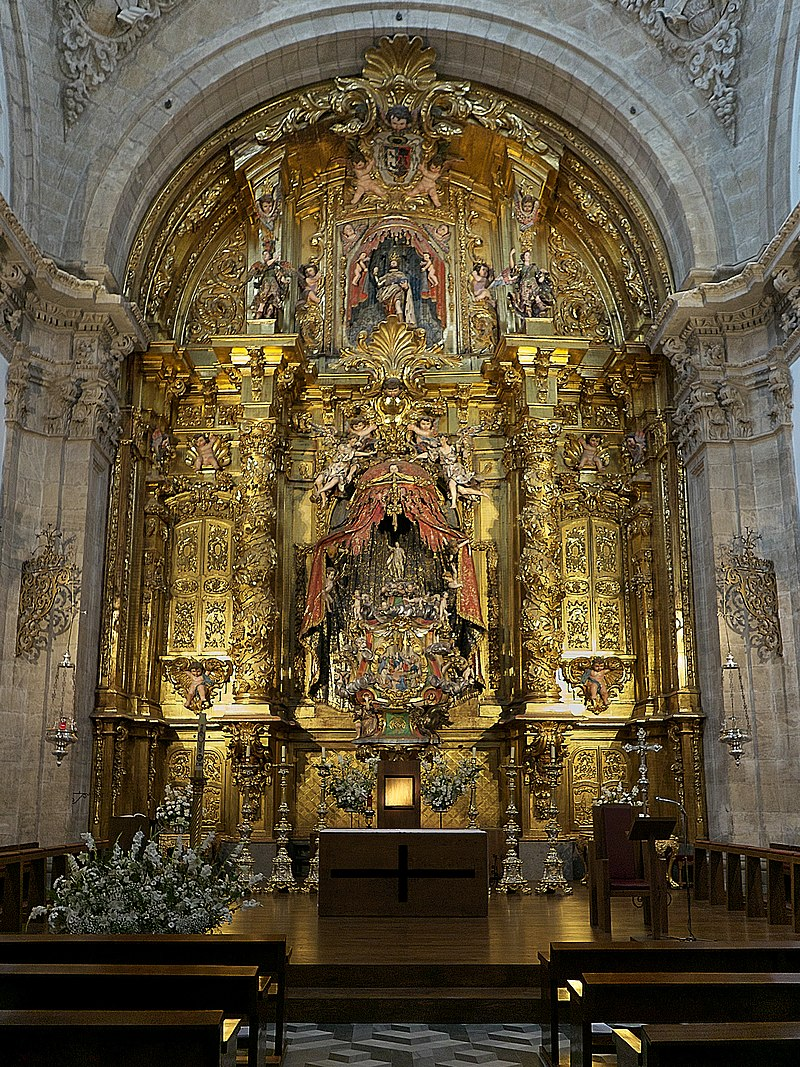
\includegraphics[scale=0.1]{ultra}
			\vskip 0.5mm
			\caption{\centering Oltár v Segovijskej Katedrále}
		\end{figure}%


	\end{columns}

\end{frame}
\begin{frame}{Klasicizmus}
	\subsection{Klasicizmus}
	\begin{itemize}
		\item Vznik : 2. polovica 18. storočia
		\item Znovuobjavenie antiky
		\item Bez výstredností baroka
		\item Stavby:
		\begin{itemize}
			\item \textcolor{BurntOrange}{Pierre-François-Léonard Fontaine} - Víťazný oblúk
			\item \textcolor{BurntOrange}{Jacques-Germain Soufflot} - Panteón
			\item \textcolor{BurntOrange}{Angel-Jacques Gabriel} - Petit Trianon
		\end{itemize}
		\begin{columns}
			\kern0pt
			\column {0.33\textwidth}
			\begin{figure}
				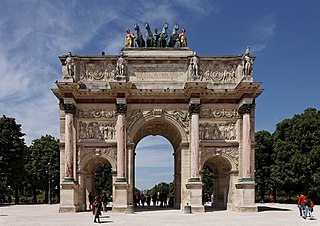
\includegraphics[scale=0.3]{ark}
				\caption{Víťazný oblúk}
			\end{figure}
			\column {0.33\textwidth}
			\begin{figure}
				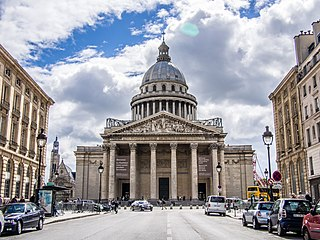
\includegraphics[scale=0.3]{panty}
				\caption{Panteón}
			\end{figure}
			\column {0.33\textwidth}
			\begin{figure}
				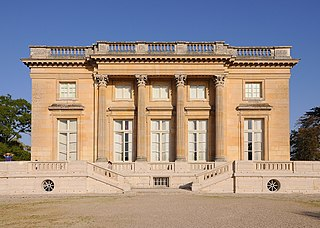
\includegraphics[scale=0.3]{maly}
				\caption{Petit Trianon}
			\end{figure}

		\end{columns}
	\end{itemize}
\end{frame}
\section{Výtvarné umenie}
\frame{\sectionpage}
\begin{frame}{Barok}
	\subsection{Barok}
	\begin{itemize}
		\item Ovplyvnené:
		\begin{itemize}
			\item Katolíckou reformou
			\item Pokrokom vo vede
		\end{itemize}
		\item Kládol sa dôraz na dramatickosť
	\end{itemize}
	\begin{columns}
		\kern0pt
		\column{0.5\textwidth}
		\begin{figure}
			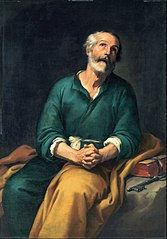
\includegraphics[scale=0.5]{slzi}
			\caption{\textcolor{BurntOrange}{B. E. Murillo}  - \textit{Svätý Peter v slzách}}

		\end{figure}%
		\column{0.5\textwidth}

		\begin{figure}
			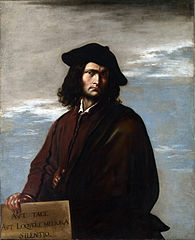
\includegraphics[scale=0.5]{filo}
			\caption{\textcolor{BurntOrange}{S. Rosa} - \textit{Filozofia}}
		\end{figure}
	\end{columns}
\end{frame}
\begin{frame}{\small \textcolor{g}{Barok} / \Large Námety}
	\subsubsection{Námety}
	\begin{itemize}
		\item Náboženské výjavy
		\item Mýtologické postavy
	\end{itemize}
	\begin{columns}
		\kern0pt
		\column{0.5\textwidth}
		\begin{figure}
			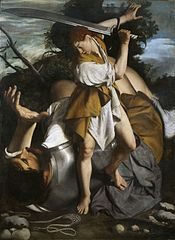
\includegraphics[scale=0.7]{golias}
			\caption{\textcolor{BurntOrange}{O. Gentileschi} - \textit{Dávid a Goliáš}}
		\end{figure}%
		\column{0.5\textwidth}

		\begin{figure}
			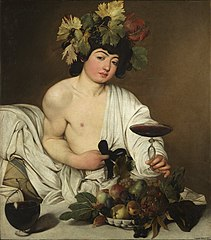
\includegraphics[scale=0.5]{pazzo}
			\caption{\textcolor{BurntOrange}{M. Caravaggio} - \textit{Bakchus}}
		\end{figure}
	\end{columns}

\end{frame}
\begin{frame}{\small \textcolor{g}{Barok} / \Large Predstavitelia}
	\subsubsection{Predstavitelia}
	\begin{itemize}
		\item Rembrandt van Rijn
		\item Jan Vermeer
		\item Anthony van Dyck
		\item Michelangelo Merisi da Caravaggio
	\end{itemize}
	\begin{columns}
		\kern0pt
		\column{0.33\textwidth}
		\begin{figure}
			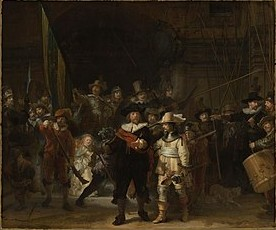
\includegraphics[scale=0.5]{hlidka}
			\vskip 1mm
			\caption{\centering \textcolor{BurntOrange}{Rembrandt} - \textit{Nočná hliadka}}
		\end{figure}%
		\column{0.33\textwidth}

		\begin{figure}
			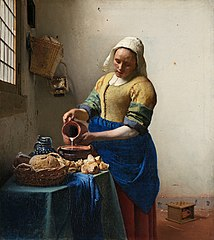
\includegraphics[scale=0.45]{milk}
			\caption{\centering \textcolor{BurntOrange}{Jan Vermeer} - \textit{Mliekarka}}
		\end{figure}%
		\column{0.33\textwidth}

		\begin{figure}

			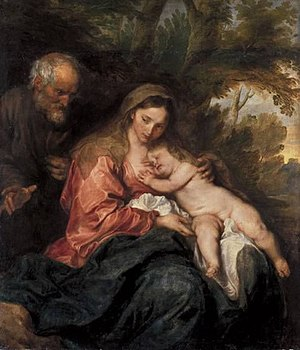
\includegraphics[scale=0.275]{oddych}
			\vskip 1mm
			\caption{\centering \textcolor{BurntOrange}{Anthony van Dyck} - \textit{Prestávka na úteku do Egypta}}
		\end{figure}
	\end{columns}
		
\end{frame}
\begin{frame}{Klasicizmus}
	\subsection{Klasicizmus}
	\begin{itemize}
		\item Vznikol vo Francúzsku
		\item Antické umenie
		\item Po objavení Pompejí
		\item Prestali sa používať náboženské výjavy
		\item Realizmus
	\end{itemize}
	\begin{columns}
		\kern0pt
		\column{0.5\textwidth}
		\begin{figure}
			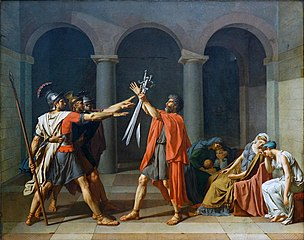
\includegraphics[scale=0.5]{horac}
			\caption{\textcolor{BurntOrange}{Jacques-Louis David} - \textit{Sľub Horáciov}}
		\end{figure}%
		\column{0.5\textwidth}
		\begin{figure}
			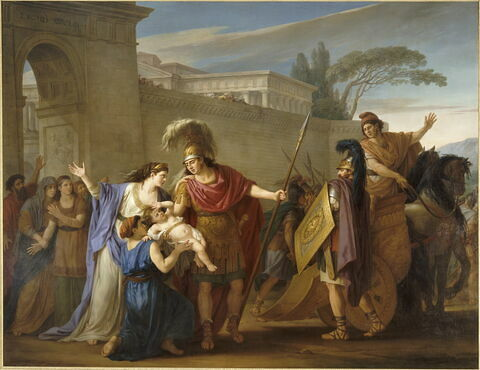
\includegraphics[scale=1.25]{og}
			\vskip 1mm
			\caption{\centering \textcolor{BurntOrange}{Joseph-Marie Vien} - \textit{Rozlúčka Hektora a Andromachy}}
		\end{figure}%

	\end{columns}
\end{frame}
\section{Kvíz}
\frame{\sectionpage}
\begin{frame}
	\subsection{Hudba}
	\textbf{HUDBA}
	\vskip 3mm
	Kto \textit{nepatril} medzi skladateľov baroka?
	\begin{columns}
	\column{0.5\textwidth}
	\begin{enumerate}
		\item J. S. Bach
		\item A. Vivaldi
		\item G. F. Händel
		\item W. A. Mozart
	\end{enumerate}
	\column{0.5\textwidth}
		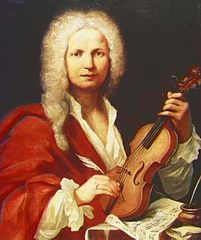
\includegraphics[scale=1.75]{vivaldi}

	\end{columns}
\end{frame}
\begin{frame}
	\textbf{HUDBA}
	\vskip 3mm
	Kto \textit{nepatril} medzi skladateľov baroka?
	\begin{columns}
	\column{0.5\textwidth}

	\begin{enumerate}
		\item J. S. Bach
		\item A. Vivaldi
		\item G. F. Händel
		\textcolor{g}{\item[\textcolor{g}{4.}] W. A. Mozart}
	\end{enumerate}
	\column{0.5\textwidth}
		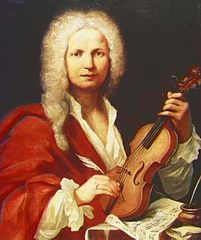
\includegraphics[scale=1.75]{vivaldi}

	\end{columns}

\end{frame}
\begin{frame}
	\textbf{HUDBA}
	\vskip 3mm
	Kto zložil \href{https://www.gtsforum.xyz/kviz1.mp3}{túto skladbu} ?
	\begin{columns}
	\column{0.5\textwidth}
	\begin{enumerate}
		\item C. Monteverdi
		\item J. Haydn
		\item L. van Beethoven
		\item N. Paganini
	\end{enumerate}
	\column{0.5\textwidth}
		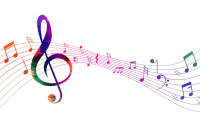
\includegraphics[scale=0.5]{music}
	\end{columns}
\end{frame}
\begin{frame}
	\textbf{HUDBA}
	\vskip 3mm
	Kto zložil \href{https://www.gtsforum.xyz/kviz1.mp3}{túto skladbu} ?
	\begin{columns}
	\column{0.5\textwidth}
	\begin{enumerate}
		\item C. Monteverdi
		\textcolor{g}{\item[\textcolor{g}{2.}] J. Haydn}\setcounter{enumi}{2}
		\item L. van Beethoven
		\item  N. Paganini
	\end{enumerate}
	\column{0.5\textwidth}
		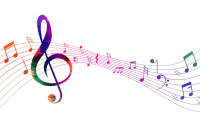
\includegraphics[scale=0.5]{music}

	\end{columns}
\end{frame}
\begin{frame}
	\subsection{Literatúra}
	\textbf{LITERATÚRA}
	\vskip 3mm
	Kto  napísal \textit{Stratený raj}?
	\begin{columns}
	\column{0.5\textwidth}
	\begin{enumerate}
		\item W. Shakespeare
		\item D. Defoe
		\item J. Milton
		\item J. Swift
	\end{enumerate}
	\column{0.5\textwidth}
		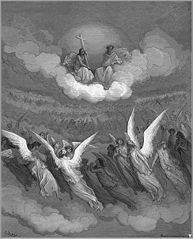
\includegraphics[scale=0.75]{lost}

	\end{columns}
\end{frame}

\begin{frame}
	\textbf{LITERATÚRA}
	\vskip 3mm
	Kto  napísal \textit{Stratený raj}?
	\begin{columns}
	\column{0.5\textwidth}
	\begin{enumerate}
		\item W. Shakespeare
		\item D. Defoe
		\textcolor{g}{\item[\textcolor{g}{3.}] J. Milton}\setcounter{enumi}{3}

		\item J. Swift

	\end{enumerate}
	\column{0.5\textwidth}
		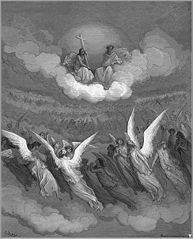
\includegraphics[scale=0.75]{lost}

	\end{columns}
\end{frame}
\begin{frame}
	\textbf{LITERATÚRA}
	\vskip 3mm
	Čo je najvýznamnejšie dielo Miguela de Cervantes?
	\begin{columns}
	\column{0.5\textwidth}
	\begin{enumerate}
		\item Don Quijote
		\item Hamlet
		\item Rozprava o Metóde
		\item Šialenstvo vo Valencii
	\end{enumerate}
	\column{0.5\textwidth}
		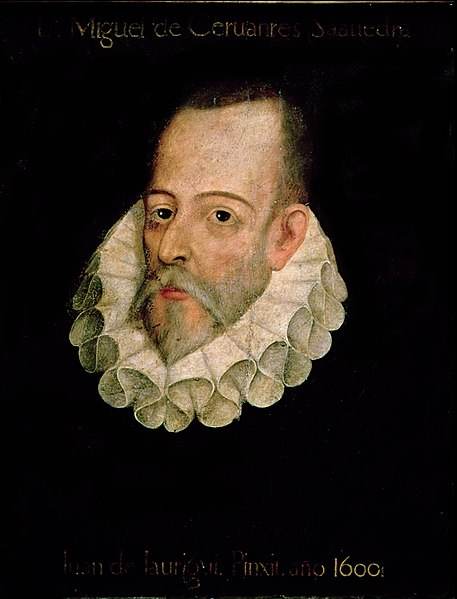
\includegraphics[scale=0.25]{cervo}

	\end{columns}
\end{frame}
\begin{frame}
	\textbf{LITERATÚRA}
	\vskip 3mm
	Čo je najvýznamnejšie dielo Miguela de Cervantes?
	\begin{columns}
	\column{0.5\textwidth}
	\begin{enumerate}
		\item[\textcolor{g}{1.}] \textcolor{g}{Don Quijote}\setcounter{enumi}{1}
		\item Hamlet
		\item Rozprava o Metóde
		\item Šialenstvo vo Valencii
	\end{enumerate}
	\column{0.5\textwidth}
		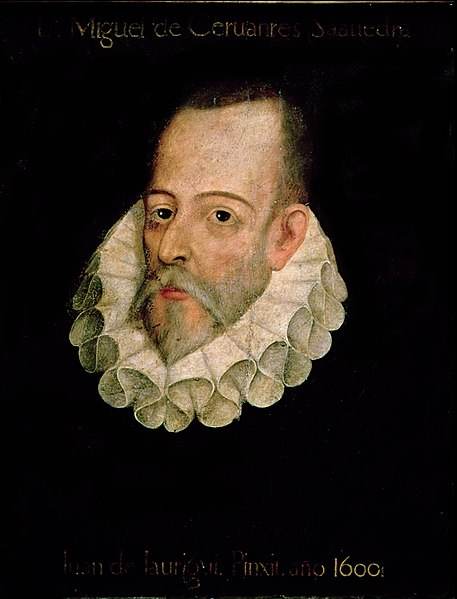
\includegraphics[scale=0.25]{cervo}

	\end{columns}
\end{frame}
\begin{frame}
	\subsection{Architektúra}
	\textbf{ARCHITEKTÚRA}
	\vskip 3mm
	V akom štýle bola postavená táto stavba?
	\begin{columns}
	\column{0.5\textwidth}
	\begin{enumerate}
		\item Skorý barok
		\item Vrcholný barok
		\item Churriguerizmus
		\item Klasicizmus
	\end{enumerate}
	\column{0.5\textwidth}
		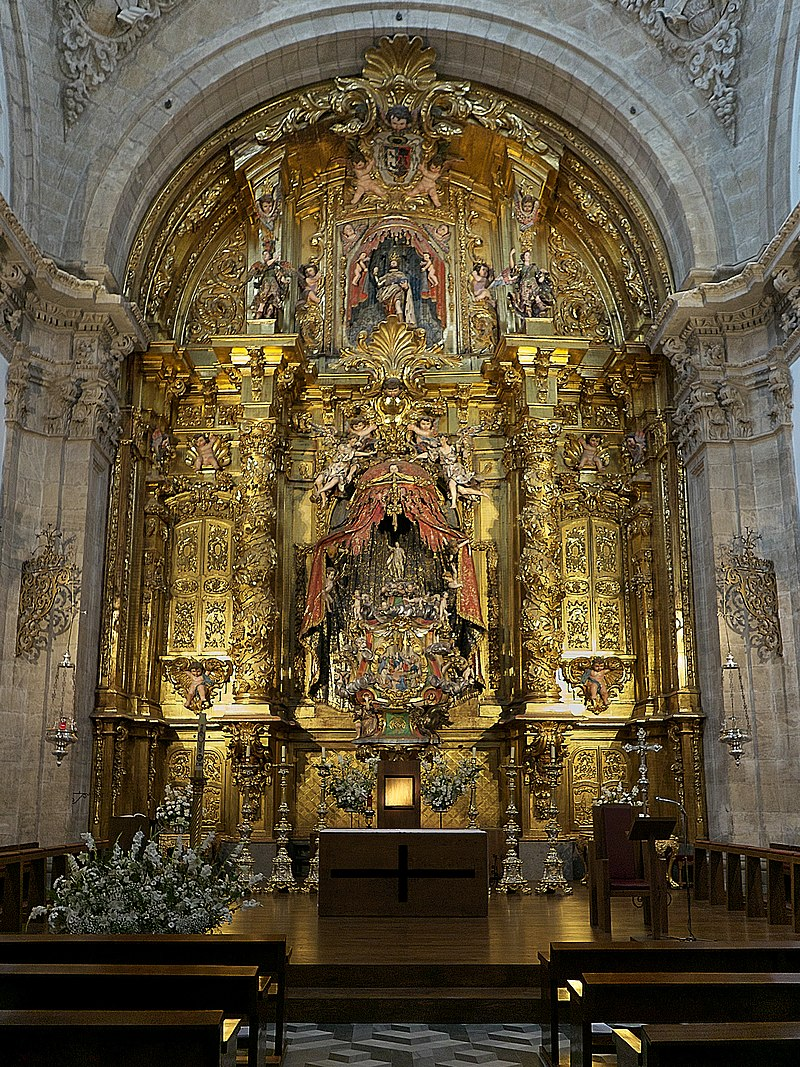
\includegraphics[scale=0.2]{ultra}

	\end{columns}
\end{frame}
\begin{frame}
	\textbf{ARCHITEKTÚRA}
	\vskip 3mm
	V akom štýle bola postavená táto stavba?
	\begin{columns}
	\column{0.5\textwidth}
	\begin{enumerate}
		\item Skorý barok
		\item Vrcholný barok
		\item [\textcolor{g}{3.}] \textcolor{g}{Churriguerizmus}\setcounter{enumi}{3}
		\item Klasicizmus
	\end{enumerate}
	\column{0.5\textwidth}
		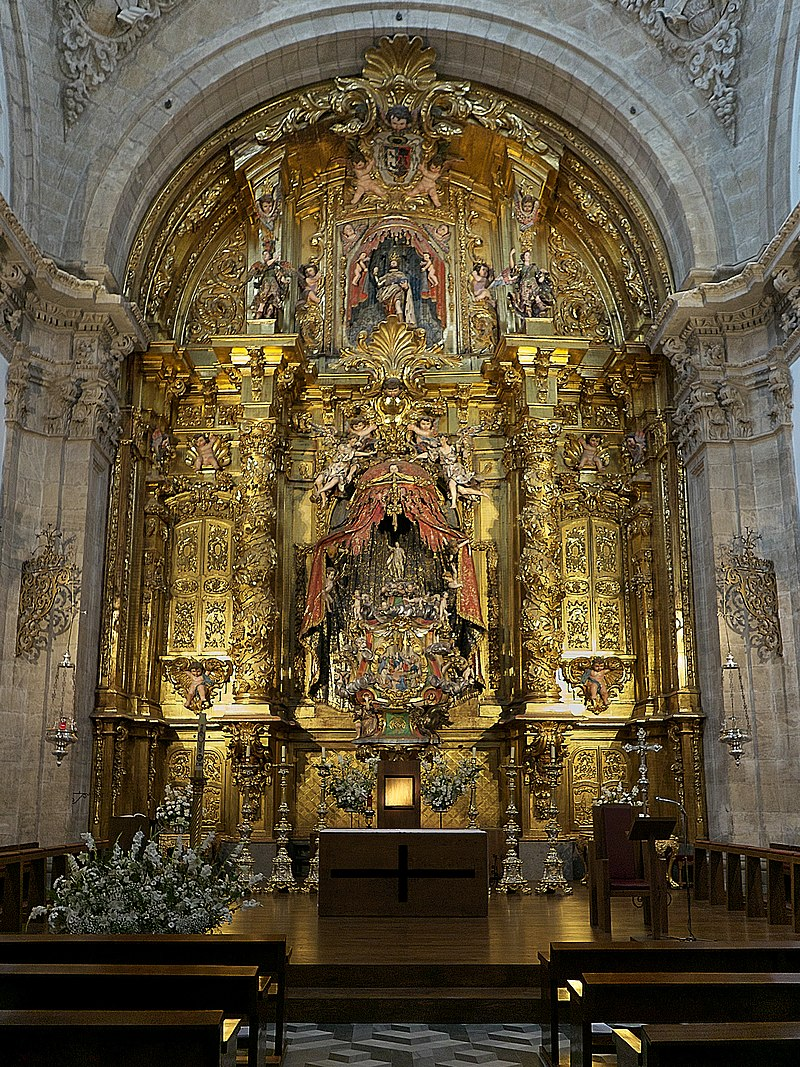
\includegraphics[scale=0.2]{ultra}

	\end{columns}
\end{frame}
\begin{frame}
	\textbf{ARCHITEKTÚRA}
	\vskip 3mm
	Kto bol hlavný cirkevný architekt počas obdobia vrcholného baroka?
	\begin{columns}
	\column{0.5\textwidth}
	\begin{enumerate}
		\item Urban VIII.
		\item Carlo Maderno
		\item Gian Lorenzo Bernini
		\item Filippo Juvarra
	\end{enumerate}
	\column{0.5\textwidth}
		\includegraphics[scale=1]{bern}

	\end{columns}
\end{frame}
\begin{frame}
	\textbf{ARCHITEKTÚRA}
	\vskip 3mm
	Kto bol hlavný cirkevný architekt počas obdobia vrcholného baroka?
	\begin{columns}
	\column{0.5\textwidth}
	\begin{enumerate}
		\item Urban VIII.
		\item Carlo Maderno
		\item[\textcolor{g}{3.}] \textcolor{g}{Gian Lorenzo Bernini}\setcounter{enumi}{3}
		\item Filippo Juvarra
	\end{enumerate}
	\column{0.5\textwidth}
		\includegraphics[scale=1]{bern}

	\end{columns}
\end{frame}
\begin{frame}
	\subsection{Výtvarné umenie}
	\textbf{VÝTVARNÉ UMENIE}
	\vskip 3mm
	Čo \textit{nevyužívalo} barokové umenie ?
	\begin{columns}
	\column{0.5\textwidth}
	\begin{enumerate}
		\item Dramatickosť
		\item Inšpiráciu antikou
		\item Mýtologické námety
		\item Biblické výjavy
	\end{enumerate}
	\column{0.5\textwidth}
		\includegraphics[scale=1]{palette}

	\end{columns}
\end{frame}
\begin{frame}
	\textbf{VÝTVARNÉ UMENIE}
	\vskip 3mm
	Čo \textit{nevyužívalo} barokové umenie ?
	\begin{columns}
	\column{0.5\textwidth}
	\begin{enumerate}
		\item Dramatickosť
		\item[\textcolor{g}{2.}] \textcolor{g}{Inšpiráciu antikou} \setcounter{enumi}{2}
		\item Mýtologické námety
		\item Biblické výjavy
	\end{enumerate}
	\column{0.5\textwidth}
		\includegraphics[scale=1]{palette}

	\end{columns}
\end{frame}

\begin{frame}
	\textbf{VÝTVARNÉ UMENIE}
	\vskip 3mm
	Kto namaľoval tento obraz?
	\begin{columns}
	\column{0.5\textwidth}
	\begin{enumerate}
		\item M. Caravaggio
		\item J. Vermeer
		\item Rembrandt
		\item J. M. Vien
	\end{enumerate}
	\column{0.5\textwidth}
		\includegraphics[scale=0.75]{pazzo}
	\end{columns}

\end{frame}

\begin{frame}
	\textbf{VÝTVARNÉ UMENIE}
	\vskip 3mm
	Kto namaľoval tento obraz?
	\begin{columns}
	\column{0.5\textwidth}
	\begin{enumerate}
		\item[\textcolor{g}{1.}] \textcolor{g}{M. Caravaggio} \setcounter{enumi}{1}
		\item J. Vermeer
		\item Rembrandt
		\item J. M. Vien
	\end{enumerate}
	\column{0.5\textwidth}
		\includegraphics[scale=0.75]{pazzo}
	\end{columns}

\end{frame}
\begin{frame}
    \begin{beamercolorbox}[sep=12pt,center]{sectionColor}%
        KONIEC\par
    \end{beamercolorbox}
\end{frame}

\begin{frame}
	\frametitle{Zdroje}
	\section{Zdroje}
	\begin{itemize}
		\large \item KNIHY
		\begin{itemize}\tiny
			\item Evans, Benjamin Ifor, a Bergonzi, Bernard. A short history of English literature. Penguin books, 1940.
			\item Briggs, Martin Shaw. Baroque architecture. TF Unwin, 1913.
		\end{itemize}
		\large \item INTERNET
		\begin{itemize}\tiny
			
			\item   \url{https://www.britannica.com/art/Western-literature/The-17th-century}%
			\item   \url{https://en.wikipedia.org/wiki/17th\_century\_in\_literature}%
			\item	\url{https://en.wikipedia.org/wiki/Spanish\_Baroque\_architecture}

			\item   \url{https://www.britannica.com/art/Neoclassical-architecture}
			\item   \url{https://beliana.sav.sk/heslo/klasicizmus}
			\item   \url{https://vytvarnavychova.sk/57-klasicizmus}
			\item   \url{https://www.britannica.com/art/Baroque-art-and-Architecture}
			\item   \url{https://classicfm.com/discover-music/periods-genres/baroque}
			\item   \url{https://baroque.org/baroque/whatis}
		\end{itemize}
	\end{itemize}
\end{frame}
\begin{frame}
    \begin{beamercolorbox}[sep=12pt,center]{sectionColor}%
        Ďakujeme za pozornosť\par
    \end{beamercolorbox}
\end{frame}
\end{document} 
